%!TEX root =  tfg.tex
\chapter{Software Product Lines}

\begin{quotation}[Novelist]{Sir James Matthew Barrie (1860--1937)}
The secret of happiness is not in doing what one likes, but in liking what one does. 
\end{quotation}

\begin{quotation}[Novelist]{Ernest Hemingway (1899--1961)}
The good parts of a book may be only something a writer is lucky enough to overhear or it may be the wreck of his whole damn life -- and one is as good as the other.
\end{quotation}

\begin{abstract}
This is an example of an abstract. Multiple lines are supported. Several paragraphs. It jumps to the next page. Blau blau blau. I am  introducing more text to reach the third line 
\end{abstract}



\section{Software Product Lines}

\begin{itemize}
\item Objective of a \Gls{pl} (mass production and customisation) \cite{benavides05-CAISE}
\item The focus in software derives in \Glspl{spl}.
\item Variability management: variability models
\item When and how are used VMs: FMs are described in FODA report as a key element in SPL since they represent the variability and commonality of the different products in a SPL.
\end{itemize}

\section{Feature Models}
\todo[inline]{To Abductive JCR Section 2.1}

As the number of products to be built by a SPL may be large and the constraints among features may be complex, representing such an information in a manageable and compact manner is a must. \fms represent the set of products a SPL may build in terms of product features. Some features are optional while others are mandatory. To indicate the relationships among features, they are hierarchically linked, forming a tree whose root is a feature representing the whole functionality of a product. The root feature is refined in child features, which increase the level of detail and reduce the scope of features. Recursively following this refinement process, a tree-like structure is obtained where three basic kinds of hierarchical relationships are used:
\begin{itemize}
\item Mandatory: a mandatory relationship affects a parent and child feature. It forces the child feature to appear in a product whenever its parent feature does. 
\item Optional: a child feature connected to a parent feature by means of an optional relationship may be optionally selected whenever its parent feature is.
\item Set-relationships: three or more features are part of a set-relationship: a parent feature and a set of two or more child features. A set-relationship contains a cardinality that constraints the number of child features to be selected in a product whenever its parent feature is selected. If the cardinality is $[1..1]$ it is commonly remarked as an \emph{alternative relationship} where only one child feature may be selected at the same time. If the cardinality is $[1..N]$ (where $N$ is the number of child features), it is also known as an \emph{or-relationship} as any combination of child features is allowed while at least one is selected.
\end{itemize}

Although \fms can represent most of the most frequent constraints, the hierarchical nature of these models might hinder the representation of some constraints. Under this circumstance, \emph{cross-tree constraints} can be added. The most common kinds of cross-tree constraints are:
\begin{itemize}
\item Dependency: a feature depends on another feature if the second one must be part of a product whenever first one is selected.
\item Exclusion: two features exclude themselves if both of them cannot be part of a product at the same time.
\end{itemize}

\begin{figure*}[htb]
	\centering
		\missingfigure{A feature model example}
		%\includegraphics[width=1.00\textwidth]{figures/reasoning.pdf}
		\caption{An example of a Home Integration System\label{fig:FMexample}}
\end{figure*}

The example in Figure \ref{fig:FMexample} describes a \emph{Home Integration System} (HIS) \spl in terms of its features and the relationships among them. Leaning on this example we define some useful terms:

\begin{description}
\item[Partial configuration] : a partial configuration is a composed by three sets of selected ($S$), removed($R$) and undecided($U$) features.  A feature can only be in one of these sets and every feature in the \fm ($fm$) must be in one of them, i.e. $S \cup R \cup U = fm$ and $S \cap R \cap U = \emptyset$. A partial configuration represents an intermediate state during the process of a customer selecting the feature for a custom product. For example, $S_P=\{...\}$, $R_P=\{...\}$ and $U_P=\{...\}$ define a partial configuration for the sample \fm where some features are still to be decided if they are to be selecter or removed in a configuration.
\end{description}

\begin{description}
\item[(Full) configuration] : a full configuration or simply a configuration is a partial configuration such that the set of undecided features in empty. For example, $S_F=\{...\}$ and $R_F=\{...\}$ describe a full configuration for the example \fm.
\end{description}

\begin{description}
\item[Product] : a product is a representation for a full configuration such that only the selected features are remarked. For instance, $P=\{\}$ is a product for the above full configuration. A product such as \texttt{A,B} is a valid since all the constraints within the \fm are satisfied. However, A,B and C is not a valid product since D is required.
\end{description}

\begin{description}
\item[Validation]
A partial configuration is \emph{valid} if all the relationships and constraints are satisfied given the sets of selected, removed and undecided features. So the definition applies for valid full configurations and valid products. As a conclusion we can affirm that a FM represents all the valid products in a SPL.
\end{description}

\objective{Briefly expose attributes as an important asset in feature models.}
It is frequent that features are not enough to represent information that is relevant to represent a \spl variability. In this case, \fms are extended with feature attributes such as cost, versions, RAM consumption, etc. in the so-called \Glspl{efm} \cite{benavides05-CAISE}. Besides relationships, an \Gls{efm} contains constraints that affect attributes which reduce even more the set of products a \fm describes. Above definitions remain when attributes are introduced into \fms. 

\section{Automated Analysis of Feature Models}

\subsection{Scope}
\todo[inline]{To Abductive JCR Intro}

FMs are used all along the SPL development as key models and many of the development decisions are taken relying on the information contained within them. Most of the times, relationships are complex and hinder the manual extraction of information. Manually obtaining information such as 'which is the product that costs the less?', 'does the feature model contain errors?' or 'why there exist no product containing certain features?' can be an unfeasible task. The complexity and compactness of FMs justify the need of an automated support of these operations. So the \textit{Automated Analysis of Feature Models} (AAFM) arises as a topic of interest to deal with this problem in the SPL community.

\sidebox{Use me to explain in a larger text than 'sidetext' anything that is important to a reader not familiar with the dissertation context for example.}

The AAFM can be seen as a black-box process that receives a FM and an operation as inputs and obtains information (its kind depends on the analysis operation) as an output (Fig. \ref{fig:oldBlackBox}). There are many operations that extract information from a FM such as 'counting products' operation whose result is a natural number indicating the number of customised products that can be built; or 'list of products' operation that obtains each of those products. This vision of AAFM as a black-box is valid for a subset of analysis operations that we call \emph{information extraction operations} (IEO) that can be seen as processes to extract information from FMs. In other words, an IEO makes explicit an implicit information within a FM. 

\begin{figure}[htb]
	\centering
	\subfigure[The AAFM seen as a black-box process]{
		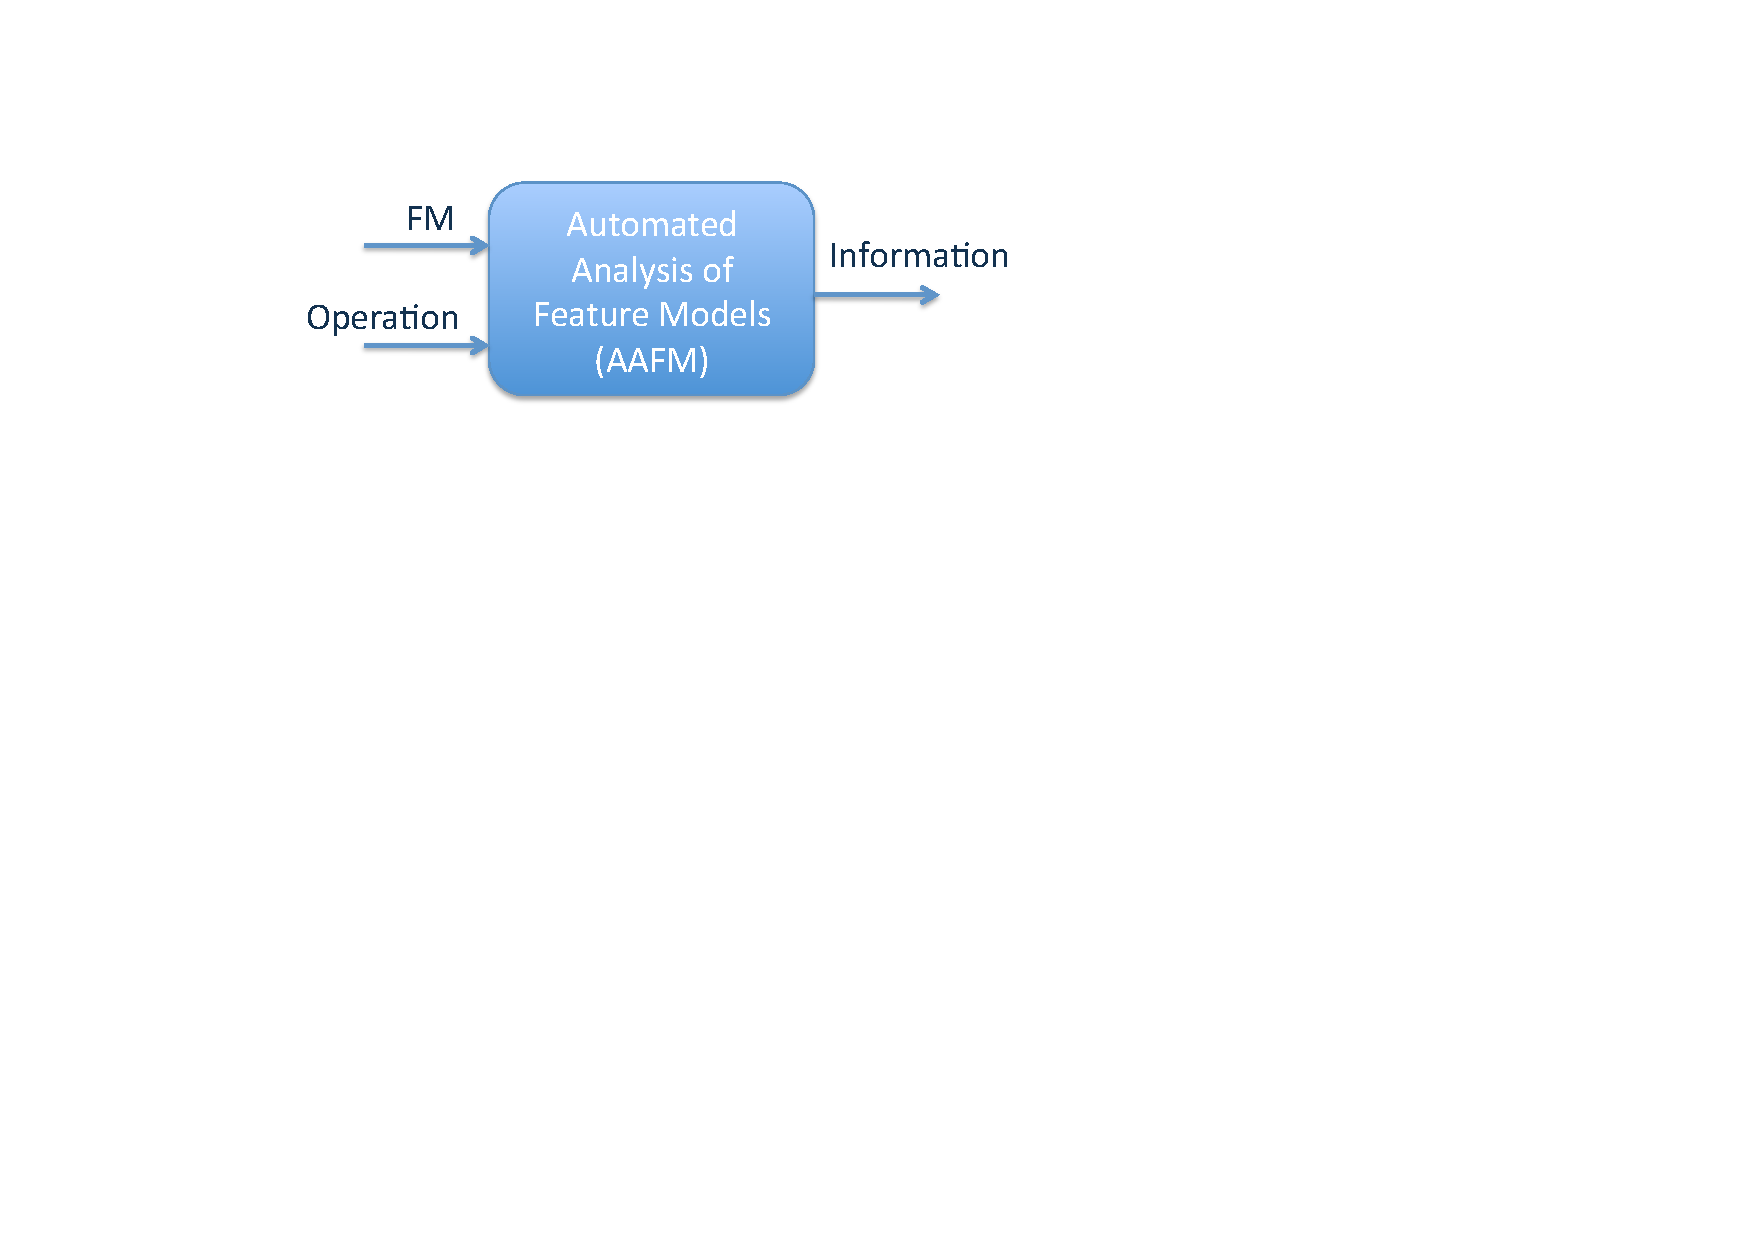
\includegraphics[width=0.30\textwidth]{figures/Introduction/oldAAFM.pdf}
		\label{fig:oldBlackBox}
	}
		\subfigure[Extending the AAFM process with explanations]{
		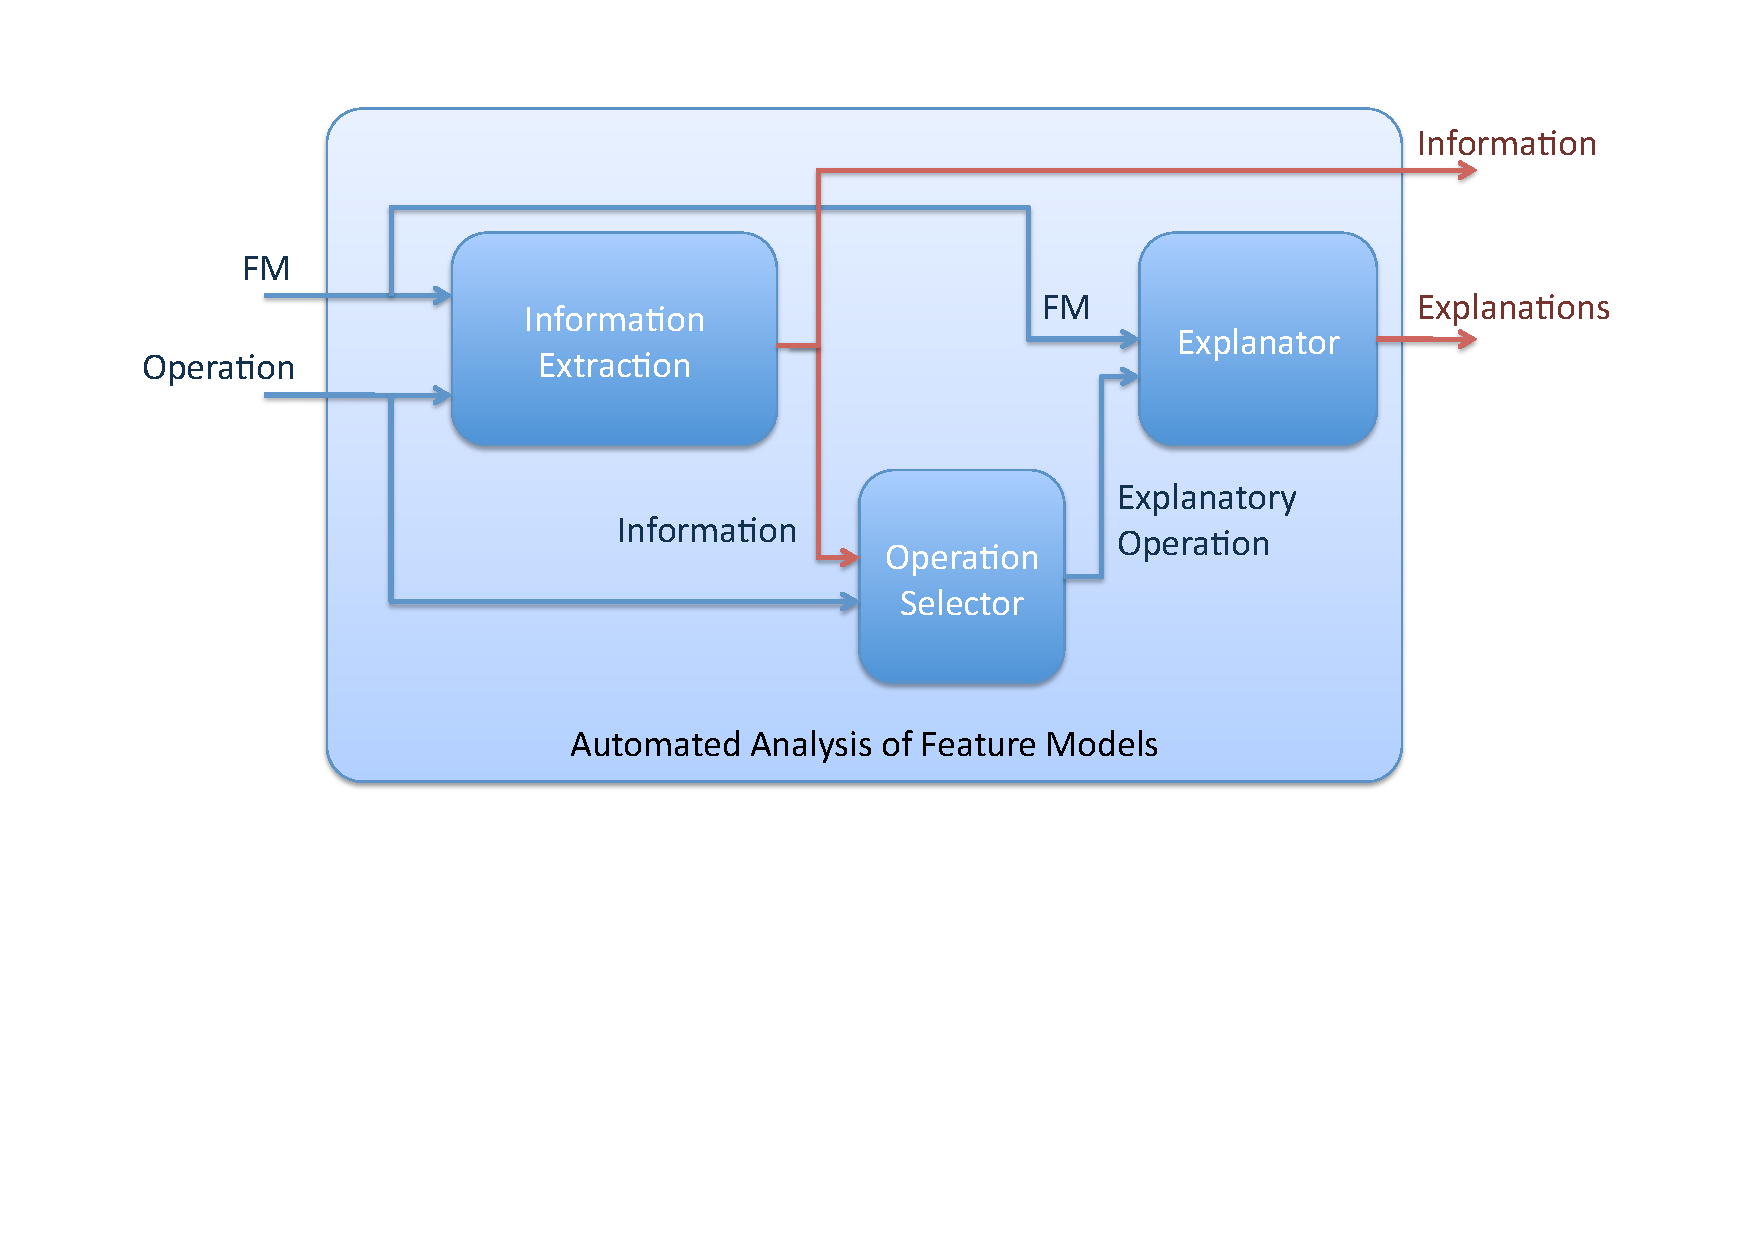
\includegraphics[width=0.65\textwidth]{figures/Introduction/newAAFM.pdf}
		\label{fig:newBlackBox}
	}
		%\missingfigure{Several architectures and a structural model for each of them (Slide 3)}
		
	\caption{A different view on AAFM distinguishing between information extraction and explanatory operations}
	\label{fig:AAFM}
\end{figure}

However, there is a subset of analysis operations known as \emph{explanatory operations} (EO) whose objective is explaining the result obtained from a IEO. Sometimes, the result is not the expected one and the analyser needs to know which are the relationships that have caused it. For example, let us suppose that the IEO 'which are the products described in a FM that cost less than \$1000?' obtains no products as a result. If we were expecting to obtain at least one product, it is important to determine the relationships in the FM that are responsible of that behaviour, so an EO 'why there is no product costing less than \$1000?' will shed light on the relationships that avoid obtaining any product. Obtaining no result is not the only case that claims for explanations. If we obtained only one product as a result and we were expecting to obtain at least 10 products, although an answer is obtained the result is unexpected and the discrepancy reasons have to be found. Moreover, explanatory operations are also useful even when an expected result is obtained, to reinforce the certainty that the result is correct. So it can be concluded that EOs complement the information an FM analyser obtains from IEOs.

The complexity of feature modelling relies on correctly setting the relationships that describe the set of products to be built in a SPL. Relationships are the only elements responsible of the results obtained in FM analysis. So an \emph{explanation} is a set of relationships that may have caused that result. While IEO provides for an unique response that is known for certain, an EO provides for a set of probable explanations to a result obtained from a IEO, being only one of them a valid explanation. It would be the analyser the one in charge of discriminating the correct explanation, maybe performing new analysis operations.

\sidetext{This is a side text. Use to remark important information}

Therefore, two kinds of operations are distinguished in AAFM: information extraction and explanatory operations. Explanatory operations have no sense without a paired information extraction operation and its result. To ensure that explanatory operations are always paired to an information extraction operation, we define a new black-box process of AAFM that incorporates explanations as an additional output (see Figure \ref{fig:newBlackBox})

\begin{enumerate}
\item Information extraction: the original process, which remains the same.
\item Operation selector: depending on the information extraction operation the analyser asks for and the information obtained as a result, this process provides the explanatory operation to be performed. In other words, it pairs an explanatory operation to an information extraction operation.
\item Explanatory analysis: provides a set of explanations from the FM and the explanatory operation.
\end{enumerate} 

The overall process can be encapsulated into a holistic black-box process which receives the FM and the information extraction operation as inputs and provides a result and explanations as outputs. It can be seen as we just add explanations as an output to the analysis process. 

To realise this view on the AAFM, we need to give details on the insides of these black-boxes. Since the information extraction process is already rigourously defined in Benavides' PhD dissertation, the purpose of this paper is defining the remaining two sub-processes. We formalise the explanatory analysis process by means of default logic and provide the criteria to implement the operation selector process.

Most Common Techniques to perform AAFM Operations.


\section{Dynamic Software Product Lines (DSPL)}
What is a \dspl. Different points of view. What is important is the automation of reconfiguration properties relying on \spl techniques.

We focus in the application of explanations in \dspls as an application of our results. Specifically we have worked in MAS and smart homes providing a solution for automating product reconfiguration.

\section{Hypothesis and Objectives}

\objective{Justifying that explanations are a particular set of operations in AAFM that are not solvable by means of the techniques that are used up-to-date}
\objective{Set an impacting phrase that summarises the hypothesis}
\importantframe{Hypothesis}{Explanations cannot be solved by AI techniques used to solve AAFM. There should exist other AI techniques to solve explanations. }

\importantframe{Objective of the dissertation}{Defining a framework to provide solutions for explanatory analysis in FMs.}

This dissertation summarises our contribution to solve some of the objectives we set in our PhD project. 

\begin{itemize}
\item Defining a catalog of analysis operations where explanations are applied.
\item Rigorously defining these operations in terms of logics.
\item Proposing solutions to these operations.
\item Validating our results by means of tools and projects where they are applied. 
\end{itemize}

Next chapter focuses on refining how we have contributed to deal with the above objectives.

A piece of code...

\begin{lstlisting}[style=javacode]
public Map<Cardinality,CardinalValue> detectWrongCardinals() {
	// any other implementation of Map can be used instead.
	Map<Cardinality,CardinalValue> result = 
		new TreeMap<Cardinality,CardinalValue>();
	for( r : relationships) {
		if (r instanceof Set) {
			Set set = (Set)r;
			Cardinality card = set.getCardinality();
			Domain dom = card.getDomain();
			for (value: dom.getValues())
				if (isWrongCardinal(card,value))
					result.put(card,value);
		}
	}
	return result;
}
\end{lstlisting}

A coolTable. Use inside a table.
\begin{table*}[h!]
	\centering
	\begin{coolTable}{lcc}{3} % 3 is the only addition to standard tabular environment
	% lcc is the alignment for each columns. 3 is the total number of columns of the table.
{A Catalog of FM Explanatory Operations (2009 version)}
			\textbf{Information Extraction Operation}&\multicolumn{2}{c}{\textbf{FM Explanatory Operations}}\\
			\midrule
			% Always use midrules instead of \hline. It adds an extra vertical space that helps to improve the clarity
			&\textit{Why? operation}&\textit{Why not? operation}\\
			\cmidrule(r){2-3} % use cmidrule instead of \cline.
			Valid FM&-&invalid FM \\
			Valid Configuration&valid partial conf.&invalid partial conf.\\		
			Valid Product&valid product&invalid product\\
			Products Listing&vaild Product/Config&invalid FM/Product/Config\\
			Products Counting&vaild Product/Config&invalid FM/Product/Config\\
			Optimisation&vaild Product/Config&invalid FM/Product/Config\\
			Core feature&core feature&core feature\\
			Variant feature&variant feature&variant feature\\
			Dead feature detection&-&dead feature\\
			False-optional feature detection&-&false-optional feature\\
			Wrong-cardinality detection&-&wrong cardinal\\
			%\multirow{2}{*}{\textbf{Information Extraction Operation}}
			\textbf{Information Extraction Operation}&\multicolumn{2}{c}{\textbf{Configuration Explanatory Operations}}\\
			\midrule
			&\textit{Why? operation}&\textit{Why not? operation}\\
			\cmidrule(r){2-3}
			Valid Configuration&valid partial conf.&invalid partial conf.\\	
		\end{coolTable}
	\caption{Most frequently used explanatory operations and their corresponding information extraction operations}
	\label{tab:listDeductiveAbductive}
\end{table*}

Use \\TableSubtitle\{n,title\} to add a subtitle as the header. n is the number of columns and title is the text to place. \citep{benavides05-CAISE}